%%%%%%%%%%%%%%%%%%%%%%%%%%%%%%%%%%%%%%%%%%%%%%%%%%%%%%%%%%%%%%%%%%%%%%
% External GPU -- Sonnet eGPU Breakaway Box 750ex field manual
% Author: Prof. Dr.-Ing. Mark Schutera
% Based on Tufte-style layout
\makeindex
%%%%%%%%%%%%%%%%%%%%%%%%%%%%%%%%%%%%%%%%%%%%%%%%%%%%%%%%%%%%%%%%%%%%%%
%
% A field manual for the lab's Sonnet eGPU Breakaway Box 750ex. Same shape
% as notes_3dprinting and notes_dgxspark: short chapters, one topic each,
% every chapter also ships as its own handout PDF under chapter_pdfs/.
%
% Facts come from Sonnet's own documentation only (egpu.bib): the tech
% specs page, the Quick Start Guide rev. D, and the Windows graphics guide.
%
% Chapter spine.
%   01 Quickstart                  -- WRITTEN, laptop check to a running external GPU
%
%%%%%%%%%%%%%%%%%%%%%%%%%%%%%%%%%%%%%%%%%%%%%%%%%%%%%%%%%%%%%%%%%%%%%%

\documentclass{../sharedAssets/tufte}

%%
% Book metadata
\title{External GPU}
\author[\defaultauthor]{\defaultauthor}
\publisher[\defaultpublisher]{\defaultpublisher}
\renewcommand{\notesdir}{notes_egpu}

% Load optional fonts
\loadoptionalfonts

% Additional packages
\usepackage{amsmath}
\usepackage{soul}
\usepackage{textcase}
\usepackage{enumitem}
\usepackage{tabularx}
\usepackage{tikz}
\usetikzlibrary{positioning,arrows.meta,fit}
\usepackage{fancyvrb}
\usepackage{float}
% Break long URLs anywhere so href'd links in the narrow Tufte margins
% wrap instead of running off the side of the page.
\usepackage{xurl}
\Urlmuskip=0mu plus 1mu\relax

% Let chapters open on any page instead of always on a recto. The shared
% class hardcodes \LoadClass[a5paper]{tufte-book} and forwards no options,
% so the flag is set here rather than passed (as in notes_3dprinting).
\makeatletter
\@openrightfalse
\makeatother

\begin{document}

\makestandardfrontmatter
\makededication{\openepigraph{``Once men turned their thinking over to
machines in the hope that this would set them free.''}{Reverend Mother
Gaius Helen Mohiam, in Frank Herbert, Dune}}
\tableofcontents

% Introduction
\makeintroduction{%
  \newthought{This is a manual.} It gets a desktop NVIDIA graphics card
  with 16~GB of memory running on your laptop through the lab's Sonnet eGPU Breakaway Box 750ex: A
  Thunderbolt enclosure with one PCIe slot, a 750~W power supply, four
  USB-A ports, and Gigabit Ethernet.
  \marginnote{\newthought{The official documentation.} Sonnet's (no, not your Claude Sonnet) product
  page carries the tech specs, the quick start guide, and the macOS and
  Windows graphics guides.\par\medskip
  \noindent\qrcode[height=1.0cm]{https://www.sonnettech.com/product/egpu-breakaway-box/overview.html}}
  Most of the work happens before you plug anything in, because most
  laptops cannot drive it. Check yours first.
  If a step in this manuel is deprecated or you found a better way, contribute it back.
  Of course feel free to add any information that you think is useful for the next person who wants to use the eGPU.

  % Flow sits centred in the free space below the text, the page ends after it.
  \vspace*{\fill}
  \marginnote{\newthought{Powerful, but} it is quite picky. Last time we looked these were the compatibility specs. Feel free to challenge and adjust the document if needed.}
  {\centering
  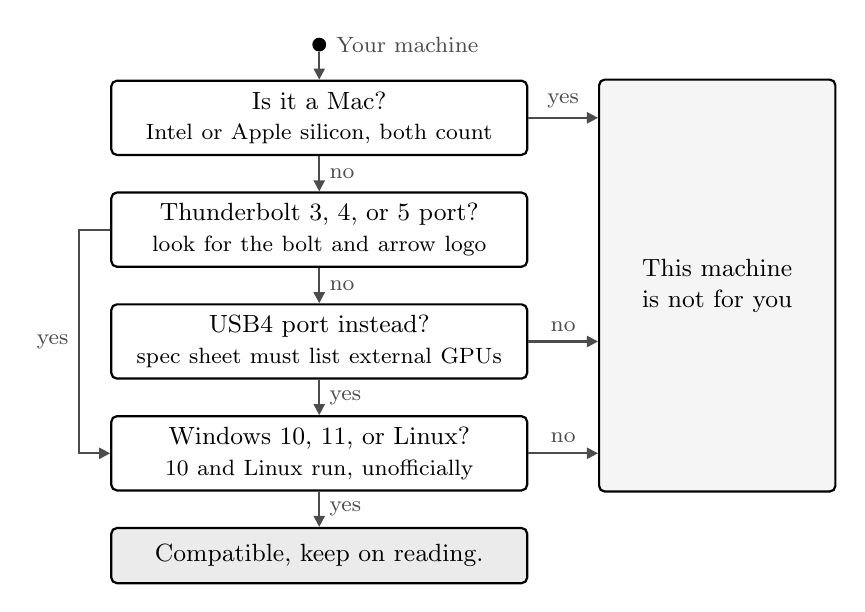
\begin{tikzpicture}[
      every node/.style={font=\small, align=center},
      ask/.style={rectangle, draw=black, thick, rounded corners=2pt,
                  text width=5cm, minimum height=0.7cm, inner sep=4pt},
      go/.style={ask, fill=black!8},
      arr/.style={-{Triangle[length=4pt, width=4pt, fill=black!70]}, thick, black!70},
      lbl/.style={font=\footnotesize, text=black!70},
    ]
    % A compatibility check only, no setup steps. The Mac question comes
    % first because it is about the hardware: with an NVIDIA card no Mac
    % passes (no macOS driver, no eGPU on Apple silicon, no Boot Camp).
    % Detailed but lenient: every question says how to tell, and only hard
    % dead ends stop a machine. Windows 10 and Linux pass although Sonnet
    % lists Windows 11 only; Sonnet's PC exceptions (early Thunderbolt 3,
    % Acer Swift TB4) are left for students to find.
    \node[circle, fill=black, inner sep=0pt, minimum size=5pt,
          label={[lbl]right:Your machine}] (start) {};
    \node[ask, below=0.35cm of start] (mac) {Is it a Mac?\\
      {\footnotesize Intel or Apple silicon, both count}};
    \node[ask, below=0.45cm of mac] (tb) {Thunderbolt 3, 4, or 5 port?\\
      {\footnotesize look for the bolt and arrow logo}};
    \node[ask, below=0.45cm of tb] (usb) {USB4 port instead?\\
      {\footnotesize spec sheet must list external GPUs}};
    \node[ask, below=0.45cm of usb] (os) {Windows 10, 11, or Linux?\\
      {\footnotesize 10 and Linux run, unofficially}};
    \node[go, below=0.45cm of os] (ok) {Compatible, keep on reading.};
    % One dead end for every failed check: a single box spanning them all.
    \path (mac.east) ++(0.9cm,0) coordinate (nx);
    \coordinate (nt) at (nx |- mac.north);
    \coordinate (nb) at ([xshift=3cm]nx |- os.south);
    \node[rectangle, draw=black, thick, rounded corners=2pt, fill=black!4,
          fit=(nt)(nb), inner sep=0pt] (no) {};
    \node[text width=2.6cm] at (no.center) {This machine\\is not for you};
    \draw[arr] (start) -- (mac);
    \draw[arr] (mac) -- node[lbl, right] {no} (tb);
    \draw[arr] (tb) -- node[lbl, right] {no} (usb);
    \draw[arr] (usb) -- node[lbl, right] {yes} (os);
    % Thunderbolt skips the USB4 question on the left.
    \draw[arr] (tb.west) -- ++(-0.4,0) |- node[lbl, left, pos=0.25] {yes} (os.west);
    \draw[arr] (os) -- node[lbl, right] {yes} (ok);
    \draw[arr] (mac.east) -- node[lbl, above] {yes} (mac.east -| no.west);
    \draw[arr] (usb.east) -- node[lbl, above] {no} (usb.east -| no.west);
    \draw[arr] (os.east) -- node[lbl, above] {no} (os.east -| no.west);
  \end{tikzpicture}\par}
  \vspace*{\fill}
  \clearpage
  }

%% Start the main matter
\mainmatter
\authorinrectoheader

% ----------------------------------------------------------------------
% Short chapters, one topic each.
% ----------------------------------------------------------------------
% !TEX root = ../notes_egpu.tex
% Chapter 1: Quickstart -- from a compatible laptop to a running external GPU
%%%%%%%%%%%%%%%%%%%%%%%%%%%%%%%%%%%%%%%%%%%%%%%%%%%%%%%%%%%%%%%%%%%%%%
%
% Whether a laptop is compatible is settled by the flow in the
% introduction; this chapter assumes it is and does not repeat the checks.
% Windows is Sonnet's supported path, Ubuntu runs unofficially, so every
% step names both.

\index{quickstart}\index{eGPU Breakaway Box}
\chapter{Quickstart}
\printchapterversion{01_quickstart}

\section{Aaaah-ah-ah-ah, aaaah-ah-ah-ah, Thunder!}
\marginnote{\newthought{The soundtrack} for first use. Meant to be played loud. Your neighbours will understand.\par\medskip
\noindent\qrcode[height=1.0cm]{https://open.spotify.com/track/57bgtoPSgt236HzfBOd8kj}}

\index{borrowing}\newthought{Lucky you.} Your machine is compatible.
Ask for the box next. You get a time slot and
hand the box back with its cable and power cord. Never attempt to open the case, and don't drop it.
\marginnote{\newthought{Scan the code} and send a mail stating your name,
course, laptop model, why and what you want to run.\par\medskip
\null\hfill\qrcode[height=1.0cm]{mailto:schutera@dhbw-ravensburg.de?subject=External\%20GPU\%20Box\&body=Name\%3A\%20\%0ACourse\%3A\%20\%0ALaptop\%3A\%20\%0AProject\%3A\%20}}

\index{driver}\newthought{Prepare the laptop before picking up the box.} I want to see it running before you will be allowed to take it with you.
On Windows, install pending updates, the newest BIOS from your laptop's
manufacturer, and the NVIDIA driver from NVIDIA's site; outdated firmware
can hide the card \cite{sonnet2023windows}. On Ubuntu, run
\texttt{sudo ubuntu-drivers install}.

\index{Thunderbolt cable}\newthought{Plug in.} Use the cable that comes with
the box, connect the power cord, and flip the switch on the back. The front
LED lights once the laptop is on. Keep the ventilator shafts clear.

\index{device approval}\newthought{Approve the device.} Windows on
Thunderbolt~3 asks once, choose \texttt{Always connect}. On Ubuntu, run
\texttt{boltctl enroll} with the device id that \texttt{boltctl list} shows.

\index{nvidia-smi}\newthought{Check the card.} \texttt{nvidia-smi} in a
terminal shows it with its 16~GB.
\marginnote{\newthought{Checks.} Nothings in Device
Manager means the driver is missing. Nothing at all means the box is not
detected: Check cable, power switch, and port.}



\index{eject}\newthought{Always eject before you unplug.} Stop every process
\texttt{nvidia-smi} lists, then on Windows use the NVIDIA eject icon in the
taskbar tray. Pulling the cable from a running card can crash the laptop.
\marginnote{\newthought{After a reconnect} on Windows, click
\texttt{Connect GPU} in the same tray icon.}


% Register the vendor documentation so the reference machinery has entries
% to resolve even while the book has a single chapter.
\nocite{sonnet2026specs,sonnet2026qsg,sonnet2023windows,sonnet2026compat}
\makestandardbackmatter{egpu}

\end{document}
